\documentclass{article}
\usepackage{graphicx} %package to manage images
\usepackage[utf8]{inputenc}
\usepackage[a4paper, total={6in, 8in}]{geometry}
\usepackage{xurl}
\title{Mocap/Phone}
\author{Pedro A. S. O. Neto}

\begin{document}

\maketitle

\section{Data}

3 dances captured by 1) MoCap and 2) Mobile phone accelerometer. Dances were captured at the same time by mocap and phone accelerometer.

\section{Stimulus}

Simple beat at 120BPMs.

\section{Pre-processing}

Second time derivative was extracted from the Mocap data. Each recording was trimmed to 30 seconds, encompassing from the beginning to the end of the audio stimulus. 

Accelerometer data from the phone was resampled to 120Hz to match the sampling rate of the mocap data. Linear interpolation was applied.

The norm of dimensions $x$, $y$ and $z$ was taken for both accelerometer and mocap data. Finally, the data was centered around zero with z-score for each dance (1, 2, and 3) and source (phone, and mocap).

Each pair of mocap and phone data was paired by means of cross correlation.

\section{Data consistency}

The correlation between mocap and phone data was assessed visually (Figure 1), and with pearson's R, which indicated correlations of $.92$, $.94$, and $.92$ for dances 1, 2, and 3, respectivelly.

\begin{figure}[t]
\noindent\makebox[\textwidth]{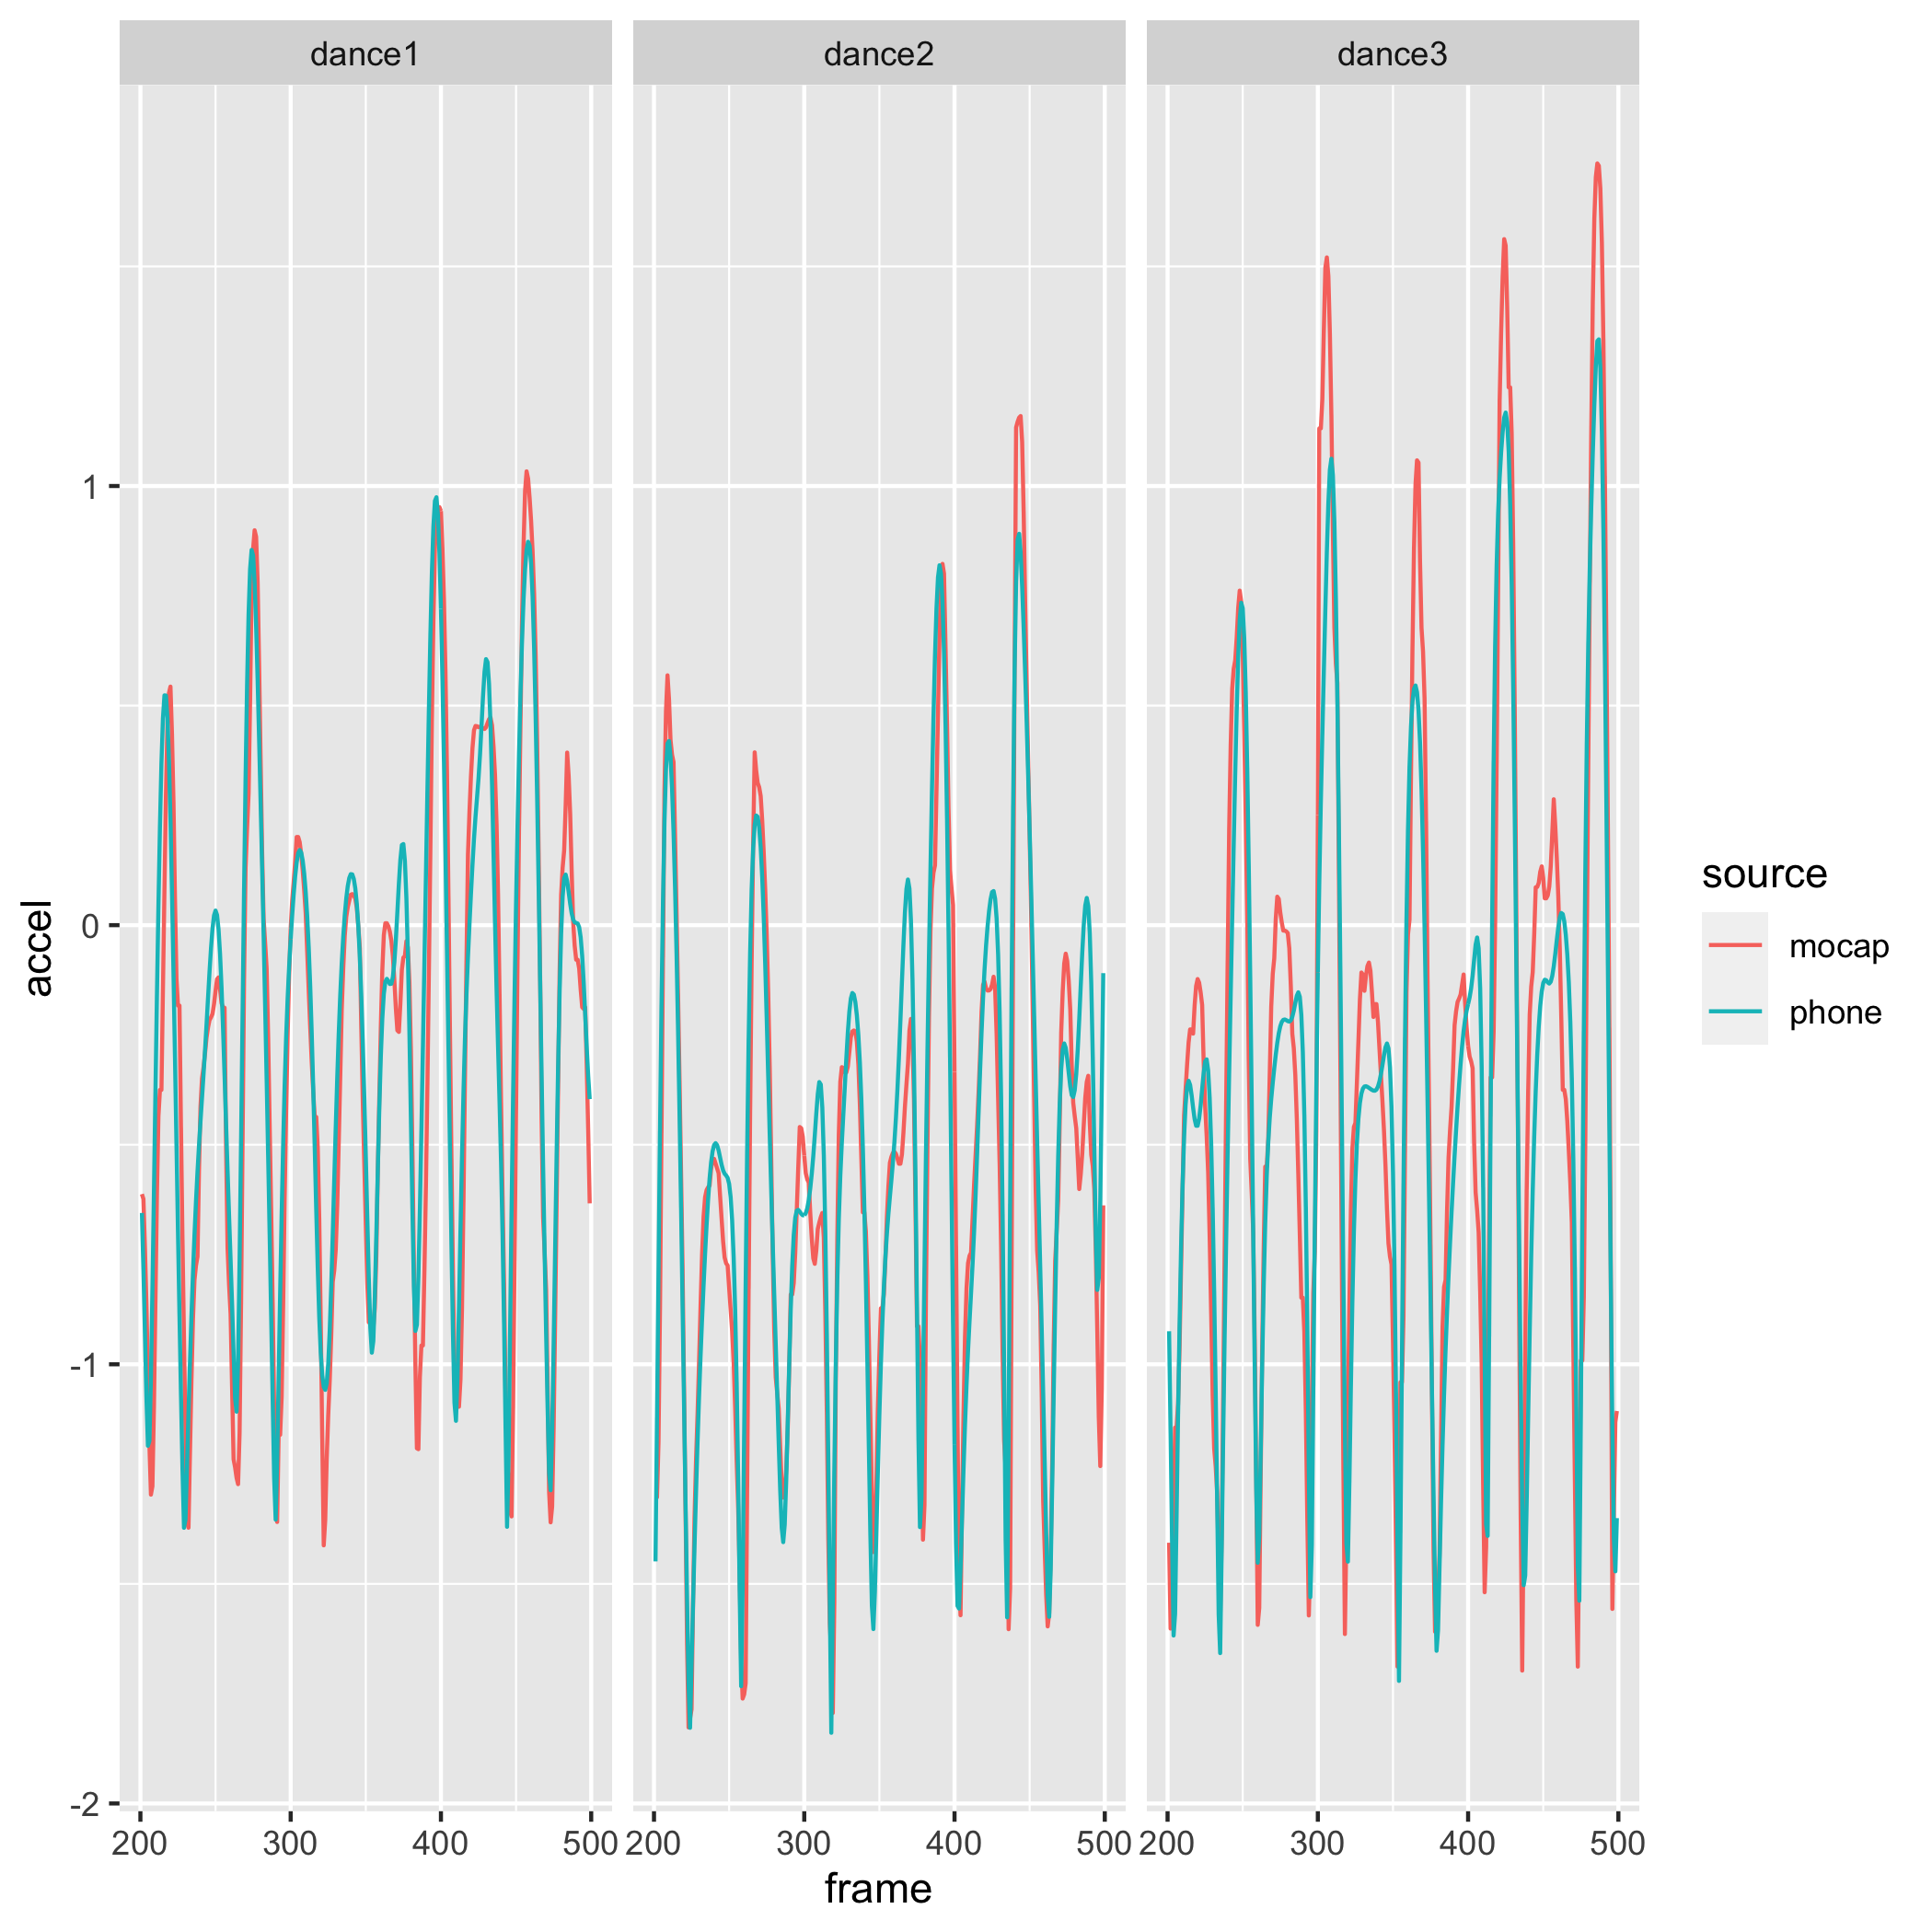
\includegraphics[width=\paperwidth]{"./accels.png"}}
\caption{Acceleration for Phone and Mocap, separated by dance}
\centering
\end{figure}

\section{Period analysis}

Each time series was divided into windows of 2 seconds, and hops of 0.25. Within each window, periodicity was extracted with an autocorelation function. Figure 2 shows the distribution of periods within each dance and within each source (phone vs mocap)

\begin{figure}[t]
\noindent\makebox[\textwidth]{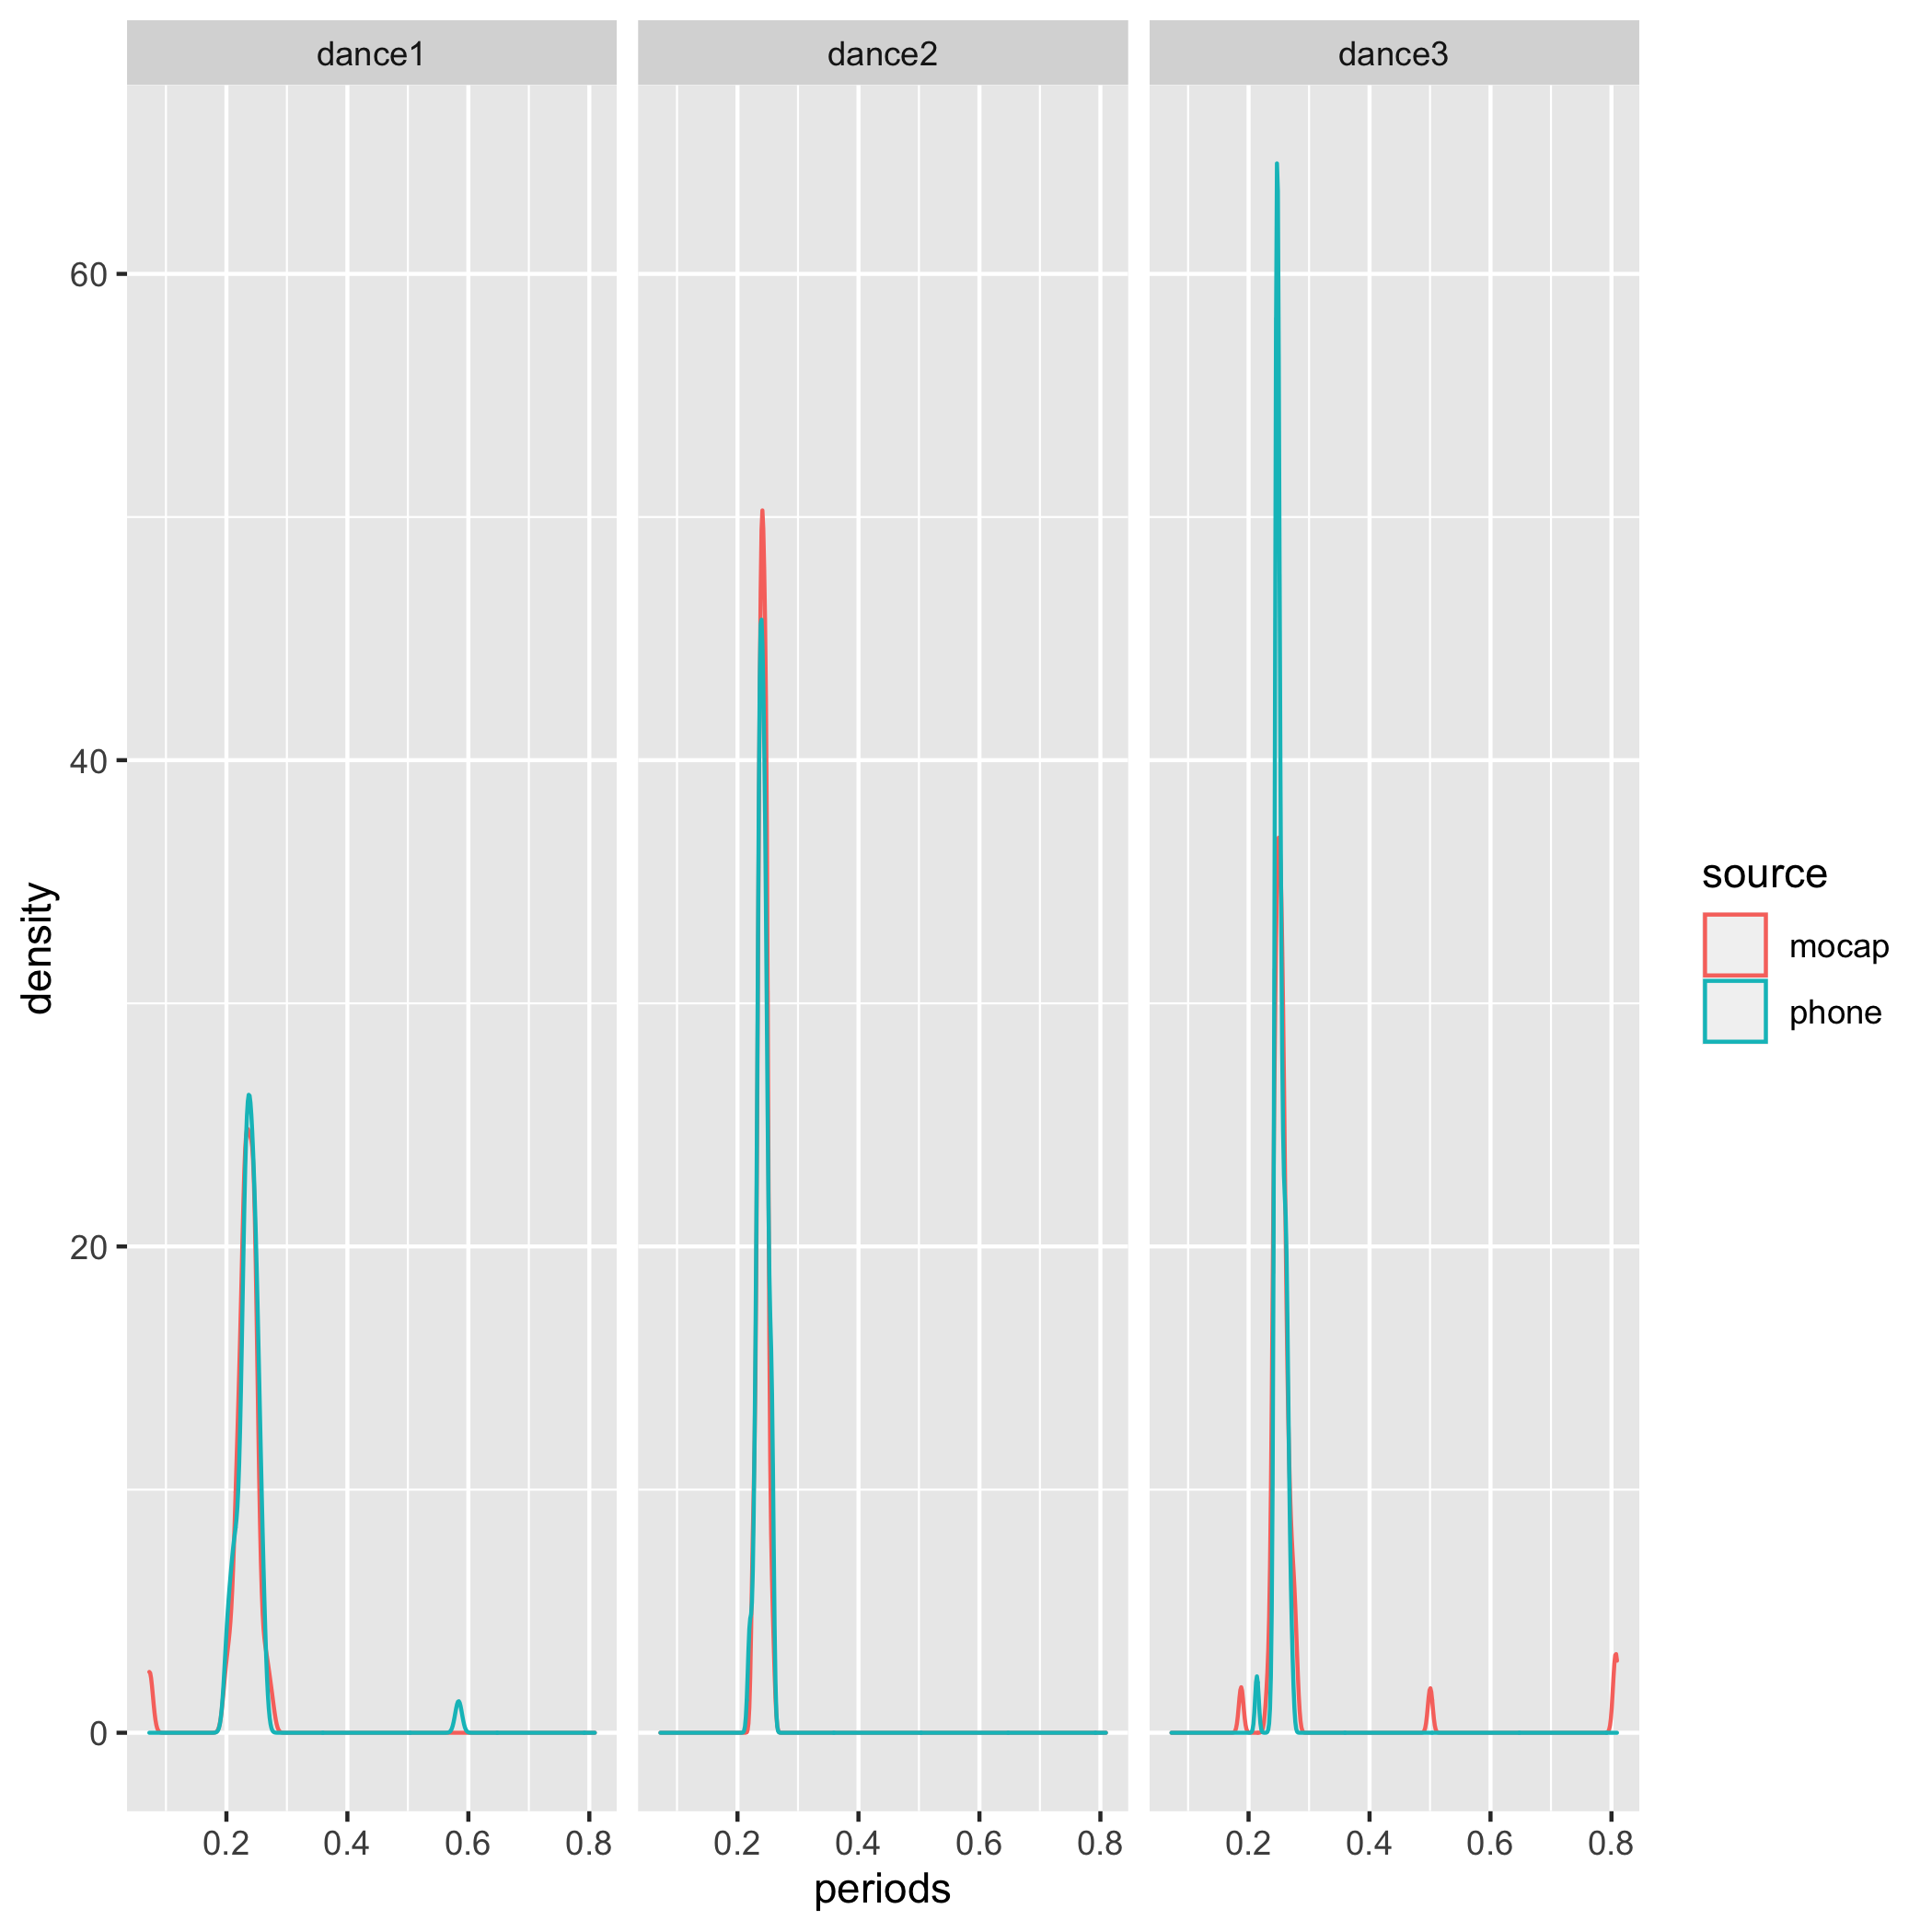
\includegraphics[width=\paperwidth]{"./periodDistribution.png"}}
\caption{Distribution of periods found for Phone and Mocap, separated by dance}
\centering
\end{figure}

To assess the consistency of windowed-periodicities between phone and mocap, I computed Pearson's r for each dance. Results indicated correlations of $0.26$, $0.56$, and $-0.26$ for dances 1, 2, and 3, respectivelly.

\begin{figure}[t]
\noindent\makebox[\textwidth]{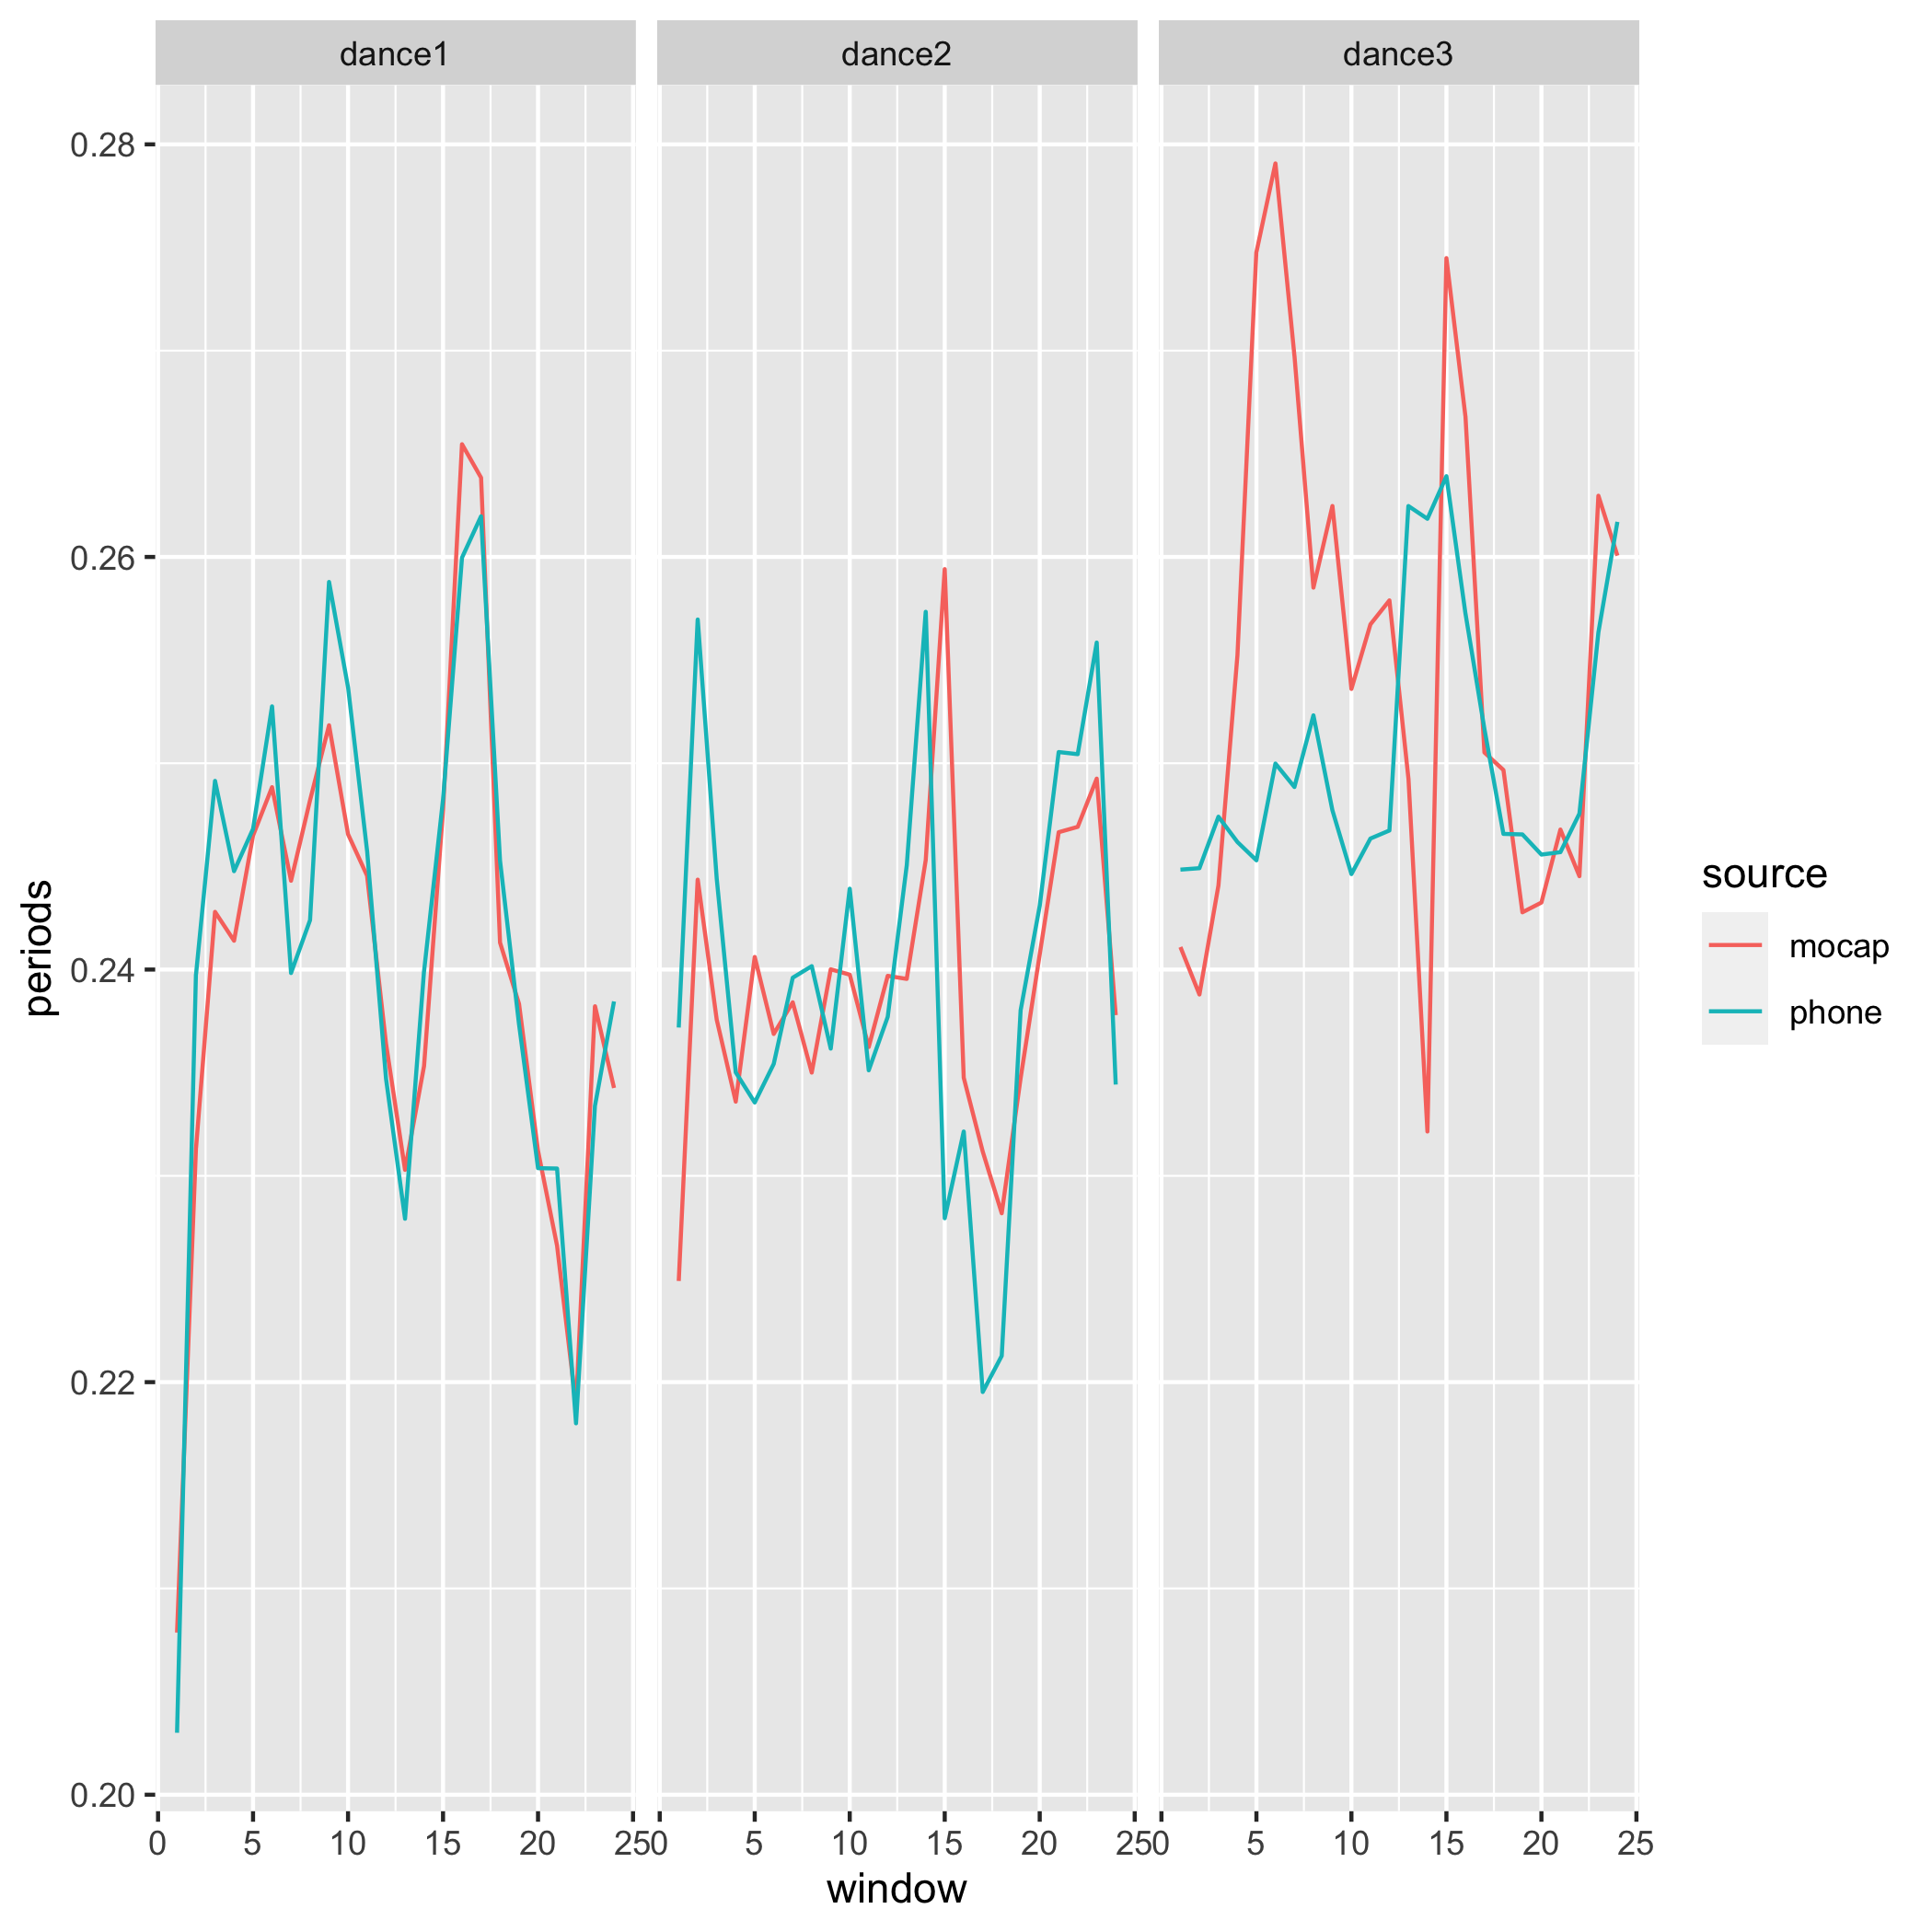
\includegraphics[width=\paperwidth]{"./periods.png"}}
\caption{Windowed periods for Phone and Mocap, separated by dance}
\centering
\end{figure}

\end{document}


